\bodychapter{Background}
\label{chp:back}

In this chapter, we provide the background necessary to understand the
    cryptographic importance of binary Edwards curves.
We begin with a brief discussion of elliptic curves in general.
Since we are mostly interested in the application of elliptic curves and
    pairing computations, we will stick to a lighter summary rather than going
    into deep mathematical detail; i.e. we will follow the example of
    \cite{washington2008elliptic} more than \cite{silverman2009arithmetic}.
We recommend these two books, along with other references in the bibliography,
    to readers interested in a more in-depth background.


\bodysection{Elliptic Curves}


\bodysubsection{Weierstrass Curves}

Broadly speaking, elliptic curves are ``curves of genus one having a specified
    base point'' (\cite{silverman2009arithmetic}).
After appropriate scaling, such curves are usually written in generalized
    Weierstrass coordinates in the homogeneous form
\[
Y^2Z + a_1XYZ + a_3YZ^2 = X^3 + a_2X^2Z + a_4XZ^2 + a_6Z^3
\]
    where $X, Y$ and $Z$ are taken to be projective coordinates from
    $\mathbb{P}^2$ over some base field $K$ and $a_1, \ldots, a_6$ are
    scalars from the algebraic closure $\overline{K}$ (though often they're
    just taken to be elements of $K$ itself).
For ease of notation, we often work in non-homogeneous affine coordinates
    instead, taking $x = \sfrac{X}{Z}$ and $y = \sfrac{Y}{Z}$:
\[
y^2 + a_1xy + a_3y^2 = x^3 + a_2x^2 + a_4x + a_6
\]
These two forms are interchangeably called the \textit{Weierstrass} form of the
    curve.
If $char(K) \notin \{2, 3\}$, then we usually simplify further to
\[
y^2 = x^3 + Ax + B
\]
    after a further change of coordinates (though of course we won't be able to
    do this when working with binary curves, i.e. curves over finite fields of
    characteristic two).
We also specify a special point, denoted by $\infty$ or $\mathcal{O}$, with the
    projective coordinates $(0 : 1 : 0)$.\footnote{We'll use $\infty$ to refer
    to this point, and reserve $\mathcal{O}$ for the neutral element on an
    Edwards curve.}
For fields $K$ with $char(K) = 2$, Weierstrass curves are usually written in
    the form
\[
y^2 + xy = x^3 + a_2x + a_6
\]

We typically only work with \textit{non-singular} curves.
That is, we don't allow the curve to have multiple roots; we choose our
    constants such that
\[
4A^3 + 27B^2 \ne 0
\]
This inequality comes from examining the discriminant of the curve in
    simplified Weierstrass form, viz. $\Delta = -16(4A^3 + 27B^2)$.
For more, see section III.1 of \cite{silverman2009arithmetic}.

If a curve is non-singular, i.e. its discriminant $\Delta$ is nonzero, then it
    indeed has genus 1 and is, if taken over the complex numbers $\mathbb{C}$,
    isomorphic to a torus.
Geometrically speaking, a non-singular curve has three distinct roots over $K$,
    so it doesn't have a \textit{cusp}---which occurs when all three roots are
    the same---or a \textit{node}---which occurs when only two of the roots are
    the same.
This will be important when we define the group law next.
See Figure \ref{fig:wc1wc2} for the graphs of two non-singular curves, and
    compare them to the graphs of the singular curves in (\ref{fig:wc3wc4}).
The first curve in Figure \ref{fig:wc3wc4} has a cusp, while the second has a
    node.

\begin{figure}[htbp]
    \mbox{
        \centering
        \subfigure[$y^2 = x^3 - 3x + 3$]{
            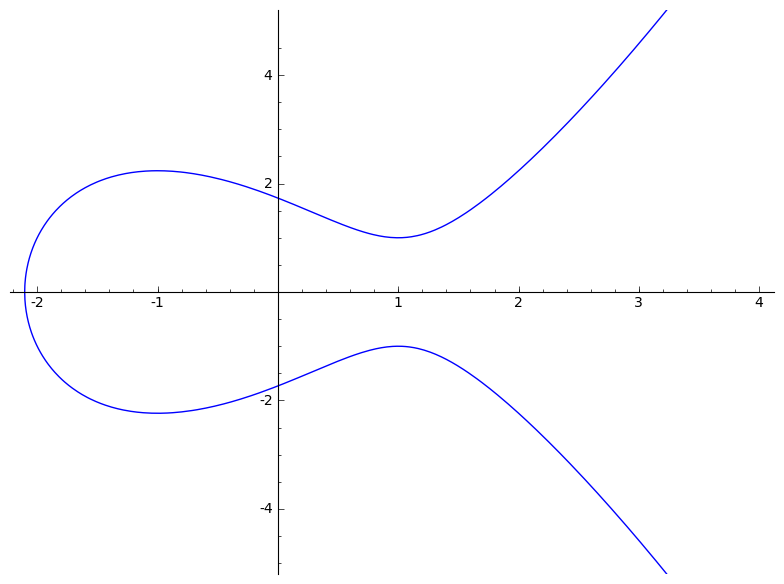
\includegraphics[scale=0.30]{figures/wc1.png}}
        \qquad\qquad
        \subfigure[$y^2 = x^3 - 2x$]{
            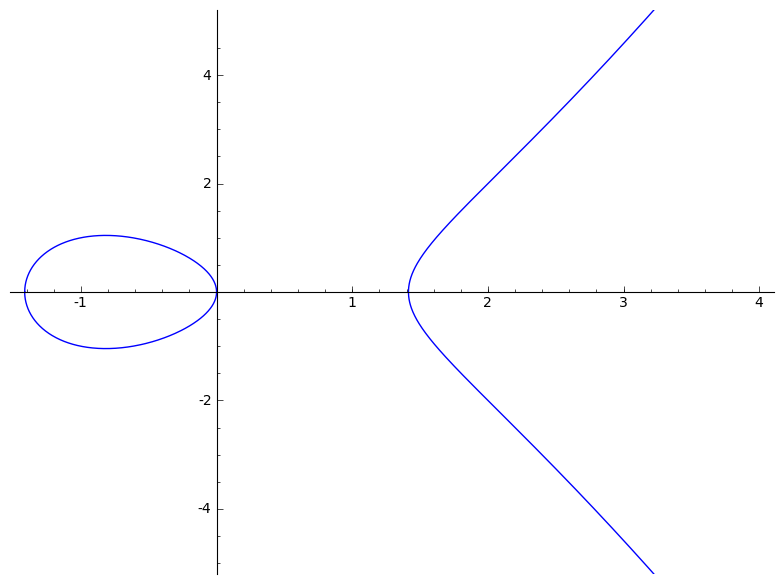
\includegraphics[scale=0.30]{figures/wc2.png}}
    }
    \caption{Two Non-singular Elliptic Curves over $\mathbb{R}$}
    \label{fig:wc1wc2}
\end{figure}

\begin{figure}[htbp]
    \mbox{
        \centering
        \subfigure[$y^2 = x^3$]{
            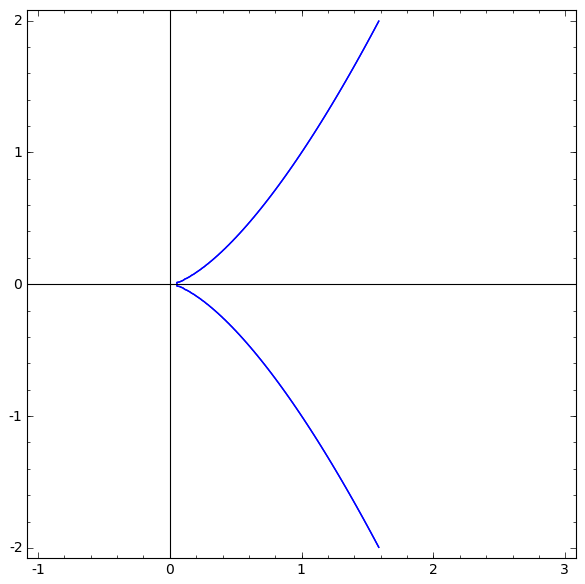
\includegraphics[scale=0.35]{figures/wc3.png}}
        \qquad\qquad
        \subfigure[$y^2 = x^3 + 2x^2$]{
            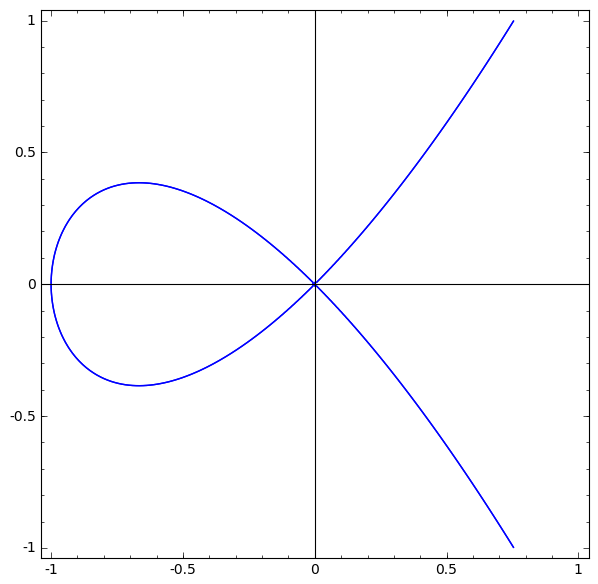
\includegraphics[scale=0.35]{figures/wc4.png}}
    }
    \caption{Two Singular Elliptic Curves over $\mathbb{R}$}
    \label{fig:wc3wc4}
\end{figure}

From here on in, we will use the notation $E(K)$ to specify an elliptic curve
    $E$ over a field $K$, or just $E$ if the field $K$ is understood.
That is,
\[
E(K) = \{\infty\} \cup \{(x, y) \in K \times K \mid 
    y^2 + a_1xy + a_3y^2 = x^3 + a_2x^2 + a_4x + a_6\}
\]
    keeping in mind that we include the ``point at infinity'' $\infty$ among
    the rational points as well.


\bodysubsection{The Group Law}

As it turns out, there's a relatively easy to understand way to define a group
    law on $E(K)$.
In this section, we'll mostly be working with $\mathbb{R}$ as our field for
    ease of notation, understanding, and graphing, but keep in mind that any
    field $K$ works just as well.
Given two points $P$ and $Q$ on $E$ over $\mathbb{R}$ with rational
    coordinates, connect them with a line; that line will (barring a few
    special cases) intersect the graph of $E$ at a third point $R^\prime$ with
    rational coordinates.
Then $R = P + Q$ is defined to be the other point where the vertical line
    through $R^\prime$ intersects the graph of $E$.
In Figure \ref{fig:wgl}, the red line connects $P$ to $Q$ on the curve
    $E: y^2 = x^3 - 3x^2 + 4$.
This line hits the curve at $R^\prime$ in the first quadrant; the green line
    connects this to $P + Q = R$.
\begin{figure}[htbp]
  \centering
  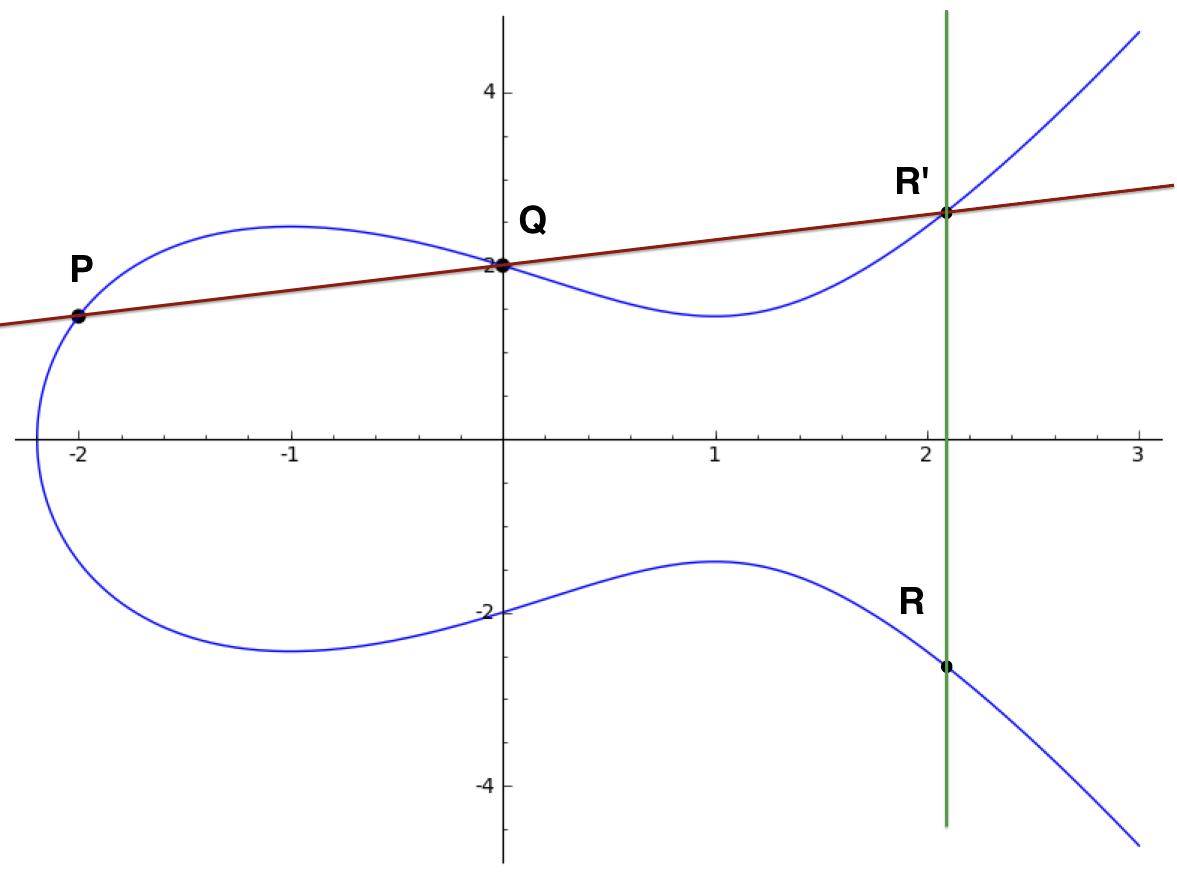
\includegraphics[scale=0.5]{figures/wgl.png}
  \caption{Weierstrass Group Law}
  \label{fig:wgl}
\end{figure}

To go from our ``chord-and-tangent'' geometric understanding to an algebraic
    one, we can use the slope of the red line (via a implicit differentiation
    of $E$'s equation, if necessary) to find $R^\prime$, then the equation of
    the curve to find $R$.
In special cases where the red line is vertical, we either have $P + (-P)
    = \infty$, the point at infinity (the identity element of our group), or $P
    + \infty = P$.
This leads us to the following for curves given in short Weierstrass form:
\begin{thm}[Weierstrass Group Law]\label{thm:wgl}
  The following formulas defining the addition of $P = (x_1,  y_1)$ and $Q =
  (x_2, y_2)$ on $E(\mathbb{R}): y^2 = x^3 + Ax + B$ turns the points
  $E(\mathbb{R})$ into an abelian group:
  \begin{enumerate}
  \item If $P = \infty$, $P + Q = Q$.
  \item If $Q = \infty$, $P + Q = P$
  \item If $x_1 \ne x_2$, $P + Q = (x_3, y_3)$ where
    \begin{displaymath}
      x_3 = m^2 - x_1 - x_2, \qquad y_3 = m(x_1 - x_3) - y_1, \qquad
      \text{ and } m = \frac{y_2 - y_1}{x_2 - x_1}
    \end{displaymath}
  \item If $x_1 = x_2$ but $y_1 \ne y_2$, $P + Q = \infty$
  \item If $P = Q$ and $y_1 \ne 0$, $P + Q = (x_3, y_3)$ where
    \begin{displaymath}
      x_3 = m^2 - 2x_1, \qquad y_3 = m(x_1 - x_3) - y_1, \qquad
      \text{ and } m = \frac{3x_1^2 + A}{2y_1}
    \end{displaymath}
  \item If $P = Q$ and $y_1 = 0$, $P + Q = \infty$
  \end{enumerate}
\end{thm}
The proof of this theorem, though not terribly difficult, is a bit tedious.
As such we will omit it, but it can be found in any text on elliptic curves or
    elliptic curve cryptography, e.g. \cite{washington2008elliptic},
    \cite{silverman2009arithmetic} (section III.2),
    \cite{koblitz2004algebraic}, \cite{cohen2005handbook}, etc.
Again, such a proof would work for any field of characteristic not equal to two
    or three; in those cases, a similar set of formulas can be found.
Of course, in finite fields our geometric understanding doesn't exactly hold
    any more---it is rather difficult to graph in $\mathbb{F}_{8675309}$, for
    example, but the algebraic structure still holds.
Similar theorems work for fields of characteristic $2$ or $3$.
One other thing to note about the above group law is that it involves a number
    of special cases; there isn't a single simple law that holds for any two
    points $P$ and $Q \in E$, and the outcome of $P + Q$ highly depends on the
    relationships between $P, Q,$ and $\infty$.
This will be important to remember when we contrast Weierstrass curves with
    Edwards curves later on.

Over a finite field $K = \mathbb{F}_q$ where $q = p^n$ for some prime $p$ and
    $n \in \mathbb{N}\setminus\{0\}$, similar algebraic work yields an abelian
    group of $\mathbb{F}_q$-rational points on $E$.
This group is very nice to work with; more precisely, we have the following
    (\cite{hankerson2004guide}'s Theorem 3.12):
\begin{thm}[Group Structure of $E(\mathbb{F}_q)$]
Let $E$ be an elliptic curve defined over $\mathbb{F}_q$.
    Then $E(\mathbb{F}_q)$ is isomorphic to the direct sum of cyclic groups
    $\mathbb{Z}_{n_1} \oplus \mathbb{Z}_{n_2}$ for some uniquely determined
    $n_1$ and $n_2 \in \mathbb{N}$ such that $n_2\vert n_1$ and $n_2 \vert
    (q-1)$.
\end{thm}
Since cyclic groups are generated by a single element, the fact that
    $E(\mathbb{F}_q)$ is isomorphic to the direct sum of two cyclic groups (or
    one, if $n_2 = 1$) make them very nice to work with computationally.
The exact details of this isomorphism are rather difficult to specify, however.
Except for specific groups that have thoroughly examined (or worked on via
    Schoof's Algorithm, see \cite{stinson2005cryptography}), the best we can
    easily find are some bounds on $\#E(\mathbb{F}_q)$, the order of the group
    $E(\mathbb{F}_q)$---even though it will of course be $n_1 \cdot
    n_2$---given by the following theorem from the 1930s:
\begin{thm}[Hasse's Theorem]
  The order of the group $E(\mathbb{F}_q)$ satisfies the inequality
  \begin{displaymath}
    q + 1 - 2\sqrt{q} \le \#E(\mathbb{F}_q) \le q + 1 + 2\sqrt{q}
  \end{displaymath}
\end{thm}

In some respects, the fact that the isomorphism $E(\mathbb{F}_q) \to
    C_{n_1} \oplus C_{n_2}$ isn't completely ironed out can seem frustrating.
However, this---along with some other aspects to be discussed shortly---is
    exactly what makes them suitable candidates for cryptographic primitives.


\bodysection{Elliptic Curve Cryptography}

In two groundbreaking papers (\cite{koblitz1987elliptic} and
    \cite{miller1986use}) Koblitz and Miller independently suggested using
    the group of rational points on an elliptic curve as the basis for a public
    key cryptosystem.
In its simplest form, elliptic curve cryptography uses the \textit{Discrete
    Logarithm Problem} and the \textit{Diffie-Hellman Problem} to hide private
    information in public.
We'll give two descriptions of the discrete logarithm problem: one in a
    multiplicative group, like $\mathbb{F}_p^\ast$, and one in an additive one
    like $E(\mathbb{F}_q)$:
\begin{prob}[DLP in multiplicative group]
Given a group $(G, \cdot)$, an element $\alpha \in G$ of order $n$, and an
  element $\beta \in \langle \alpha \rangle$, find the unique element $k \in
  \mathbb{Z}_n$ such that $\alpha^k = \beta$.
\end{prob}
\noindent We'll borrow \cite{stinson2005cryptography}'s notation and say that
    $k = \log_\alpha \beta$.

\begin{prob}[DLP in additive group]
Given a group $(G, +)$, an element $\alpha \in G$ of order $n$, and an element
  $\beta \in \langle \alpha \rangle$, find the unique element $k \in
  \mathbb{Z}_n$ such that $k\alpha = \beta$.
  \end{prob}

As \cite{stinson2005cryptography} says, ``The utility of the Discrete Logarithm
    problem in a cryptographic setting is that finding discrete logarithms is
    (probably) difficult, but the inverse operation of exponentiation can be
    computed efficiently.''
While this description favors multiplicative groups, the idea is the same in an
    additive one: repeated applications of the group operation are (relatively)
    simple to compute, but taking the result of such a computation and trying
    to find the input that yields it is (believed to be) rather difficult.
We'll say more on the ``believed to be'' qualification shortly.

ElGamal cryptosystems are based on the apparent difficulty of the following
problem, first proposed in \cite{diffie1976new}:
\begin{prob}[DHP in multiplicative group]
Given a group $(G, \cdot)$, an element $\alpha \in G$ of order $n$, and two
  elements $\beta = \alpha^b$ and $\gamma = \alpha^c$ in $\langle \alpha
  \rangle$ for some integers $b, c \in \mathbb{Z}_n$, find $\delta =
  \alpha^{bc}$.
\end{prob}
\begin{prob}[DHP in additive group]
Given a group $(G, +)$, an element $\alpha \in G$ of order $n$, and two
  elements $\beta = b \alpha$ and $\gamma = c \alpha$ in $\langle \alpha
  \rangle$ for some $b, c \in \mathbb{Z}_n$, find $\delta = (bc)\alpha$.

\end{prob}
It's apparent that should one find a fast algorithm to compute discrete logs,
    the Diffie-Hellman Problem will also be rather simple to find---once
    $\log_\alpha \beta$ and $\log_\alpha \gamma$ are found, $\delta$ can be
    computed from these two values, since
\[
\delta = \alpha^{bc} = \alpha^{(\log_\alpha \beta)(\log_\alpha \gamma)}
\]
    in multiplicative notation, or
\[
\delta = (bc)\alpha = [(\log_\alpha \beta)(\log_\alpha \gamma)]\alpha
\]
    in additive notation.
Hence the DHP is no harder than the DLP; in many groups, it is believed to be
    as difficult.

The above exposition of the Diffie-Hellman problem is also called the
    \textit{Computational Diffie-Hellman Problem}, to contrast it with the
    \textit{Decisional Diffie-Hellman Problem}:
\begin{prob}[DDHP in additive group]
Given a triple $(\beta, \gamma, \delta)$ from a group $(G, +)$ of order $n$
    such that $\beta = b \alpha$ and $\gamma = c \alpha$ for some $b, c$ chosen
    independently at random from $\mathbb{Z}_n$, determine which of the
    following two cases hold:
\begin{enumerate}
\item   $\delta = (bc)\alpha$
\item   $\delta = d\alpha$ for some other $d$ chosen at random from
    $\mathbb{Z}_n$ independently from $b$ and $c$.
\end{enumerate}
\end{prob}
This problem seems easier to solve at first blush than its computational
    counterpart, but is still rather difficult in many settings.
We rely upon the difficulty of this problem to construct a cryptosystem in
    Chapter \ref{chp:app}.

We now describe how these problems are used for the ElGamal public key
    cryptosystem in $\mathbb{F}_p^\ast$ using two favorite characters from
    cryptographic literature: Alice and Bob.\footnote{The following exposition
    is Cryptosystem 6.1 from \cite{stinson2005cryptography}.}

\begin{cryp}[ElGamal over $\mathbb{F}_p^\ast$]
Suppose Alice wishes to set up a secure way for Bob to send her a message.
They first agree on a large prime $p$ and a group element $\alpha \in
    \mathbb{F}_p^\ast$ that is a generator of the cyclic subgroup of quadratic
    residues (i.e. the set of $\gamma$ for which $\exists \beta \in
    \mathbb{F}_p^\ast$ such that $\beta^2 = \gamma$; this requirement is
    conjectured to equate the semantic security of the
    cryptosystem to solving the DLP).
Next, Alice chooses an integer $a$ (reduced modulo the order of $\alpha$) as
    her secret key and publishes $\alpha$ and $\beta = \alpha^a$.

To send a message (that's been encoded as an integer $m < p$ in some public
    fashion) securely to Alice, Bob chooses a secret integer $b$, computes
\[
(\gamma, \delta) = (\alpha^b, m\beta^b)
\]
    and transmits them to Alice.

Once she has the pair $(\gamma, \delta)$, Alice computes
\[
\delta(\gamma^a)^{-1}
    =   (m\beta^b)(\alpha^{ab})^{-1}
    =   m\alpha^{ab}\alpha^{-ab}
    =   m
\]
    and recovers the message.
\end{cryp}

The security of this system, as mentioned above, is conjectured to be
    equivalent to the feasibility of solving the discrete logarithm problem in
    this group.
That is, this system is secure as long as computing $a$ from $\alpha$ and
    $\beta$ is difficult.
To achieve this, \cite{stinson2005cryptography} states that because of rather
    efficient methods (subexponential time, but not polynomial time) for
    computing $\log_\alpha \beta$ in $\mathbb{F}_p^\ast$ like the index
    calculus algorithm, ``$p$ needs to be at least $2^{1880}$'' for this system
    to securely hide message until the year 2020.\footnote{
        \cite{stinson2005cryptography} was published in 2005.}
As we'll see, the DLP is currently much more secure in $E(\mathbb{F}_q)$ for
    much smaller key sizes.

In elliptic curve cryptography, the size of our finite field $q = p^n$ for some
    prime $p$, the details of the curve $E$, and a special point $P$ are chosen
    in a manner such that the order of $P$ is a prime equal to $\sfrac{\#E}{h}$
    for some small cofactor $h = 1, 2,$ or $4$.
Typically $q = p$ (so $n = 1$) if $p$ is a large odd prime, while $n$ is chosen
    large in the binary case where $p = 2$; see \cite{gallagher09fipspub} for
    more details.
As above, Alice chooses a secret $a$ (reduced modulo $P$'s order) and publishes
    both $P$ and $Q = aP$.

However, implementers of elliptic curve cryptography are currently able to
    choose much smaller parameters than there counterparts in other settings,
    as \cite{stinson2005cryptography} explains:
\begin{quote}
In order for an elliptic curve discrete logarithm based cryptosystem to be
    secure until the year 2020, it has been suggested that one should take $p
    \approx 2^{160}$ [if $p$ is odd] (or $n \approx 160$ [if $p = 2$]).
In contrast, $p$ needs to be at least $2^{1880}$ [in the $F_p^\ast$ case] to
  achieve the same (predicted) level of security.
The reason for this significant difference is the lack of a known index
    calculus attack on elliptic curve discrete logarithms.
\end{quote}
Because the faster DLP algorithms in $\mathbb{F}_p^\ast$ are too specialized to
    work in $E(\mathbb{F}_q)$, would-be attackers are (currently) forced to use
    more generalized algorithms that are much slower, viz. exponential in the
    bit-length of our parameters.
The following table from \cite{agency2009lr} describes the state of affairs as
of 2009:
\begin{table}[htbp]
  \centering
  \begin{tabular}[htbp]{| c | c | c |}
    \hline
    Symmetric Key & RSA \& Diffie-Hellman Key & Elliptic Curve Key\\
    \hline
    80 & 1024 & 160\\
    112 & 2048 & 224\\
    128 & 3072 & 256\\
    192 & 7680 & 384\\
    256 & 15360 & 521\\
    \hline
  \end{tabular}
  \caption{NIST recommended key sizes (measured in number of bits)}
  \label{tab:nrks}
\end{table}

As you can see from table (\ref{tab:nrks}), elliptic curves provide a strong
    alternative to other primitives for public key cryptosystems.
They can make use of this speed and ease of implementation in the following
    cryptosystem to securely share a session key for, say, a communication via
    a faster symmetric system like AES \cite{daemen2002design}:
\begin{cryp}[Diffie-Hellman Key Exchange]
Suppose Alice and Bob wish to construct a secret key with which they can
    communicate privately.
To start, they select a finite field $\mathbb{F}_q$ and a curve
    $E: y^2 = x^3 + Ax + B \bmod p$ (again, $p > 3$).
They also agree on a generator $P$ of a large subgroup $\langle P \rangle$ of
    $E(\mathbb{F}_q)$.

On her own, Alice selects a secret random element $a \in \mathbb{F}_q$ and
    computes $aP = (x_a, y_a)$ and sends it to Bob over an unsecured channel.
Likewise, Bob picks a secret $b$ and computes $bP = (x_b, y_b)$ and sends it to
    Alice.
Then, since $a(bP) = b(aP)$, they now have a shared secret key with which to
    communicate.

Moreover, an eavesdropper (Eve, say) would need either $a$ or $b$ to be able to
    recover their shared key.
However, all Eve can see is $aP$ and $bP$, so she'd need to compute a discrete
    logarithm to recover $a$ or $b$ from these multiples of $P$.
If instead she hopes to compute $abP$ from $aP$ and $bP$, she needs to solve
    the Diffie-Hellman problem, which is also believed to be quite difficult.
\end{cryp}

We conclude this section with an example of using elliptic curves for a
    Diffie-Hellman key exchange.
Computations in this section were done with the help of the Sage computer
    algebra system \cite{sage}.

\begin{ex}
To start, they follow \cite{gallagher09fipspub}'s recommendations and select
    their finite field to be $\mathbb{F}_p$ where
\[
p =  6277101735386680763835789423207666416083908700390324961279
\]
    is a prime of bit length 192.
They then pick their curve $E$ to be $y^2 = x^3 - 3x + B \bmod p$, where
\[
B = 2455155546008943817740293915197451784769108058161191238065
\]
Then per \cite{gallagher09fipspub} their generator $P$ is the point $(x, y)$,
    where
\begin{align*}
x &= 602046282375688656758213480587526111916698976636884684818\\
y &= 174050332293622031404857552280219410364023488927386650641
\end{align*}
Alice selects her secret random element $a \in \mathbb{F}_p$ to be
\[
a = 5599623221253947648338288897360753975761411887111443672469
\]
She then computes $a P = (x_a, y_a)$ where
\begin{align*}
x_a &= 5920503522293796254308104329764746582035708243035924352637\\
y_a &= 4916733057056312203451479844149885752636863324862895552670
\end{align*}
    and sends it to Bob (over an unsecured channel).
Likewise, Bob selects the secret random $b \in \mathbb{F}_p$ where
\[
b = 2188359882031140101779611982450016865481691553092225796933
\]
    and sends $b P = (x_b, y_b)$ to Alice, where
\begin{align*}
x_b &= 763794420572335512449180732023082145057259616577775194615\\
y_b &= 679692871035831936640161559745188598378636802338357105905
\end{align*}
Their shared key is now
\begin{align*}
x   &=  1714835006422896682007668925679643931430048350714705849982\\
y   &=  4464950417588212505755764847617981239405229107427517838554
\end{align*}

Here's the transcript of a \texttt{Sage} session for this
    computation:\footnote{Note that the calls to \texttt{K.random\_element()}
    will in all likelihood yield different values for $a$ and $b$ than those
    given above.}
\lstinputlisting[caption={Diffie-Hellman Example},language=Python]{listings/dh.sage}
The hexadecimal strings for $B$, $x$, and $y$, along with the choice of $p$,
    are all given in \cite{gallagher09fipspub}.
\end{ex}

\bodysection{Edwards Curves}

Inspired by studying the work of Euler and Gauss, Edwards found a new normal
    form of elliptic curves in his 2007 paper \cite{edwards2007normal}.
``In notes published posthumously in his \textit{Werke},'' writes Edwards,
    ``Gauss stated explicitly the formulas Euler had hinted at earlier'' for an
    explicit addition formula on the curve $x^2 = y^2 + x^2y^2 = 1$ which
    related to the integral 
\[
\int \frac{dx}{\sqrt{1 - x^4}}
\]
    Gauss was studying via the change of coordinates $z = y(1 + x^2)$.
Gauss wrote the formulas as
\[
S = \frac{sc^\prime + s^\prime c}{1 - ss^\prime cc^\prime}
\qquad\qquad
C = \frac{cc^\prime - ss^\prime}{1 + ss^\prime cc^\prime}
\]
As Edwards notes in \cite{edwards2007normal}, ``Gauss's choice of the letters
    $s$ and $c$ brings out the analogy with the addition laws for sines and
    cosines.''
Edwards generalized these laws to the curve
\begin{equation}
\label{eq:Ed1}
x^2 + y^2 = a^2 + a^2x^2y^2
\end{equation}
    over a field $K$ where $a \in K$ is a constant such that $a^5 \ne a$.
An example of a curve of this type is given in Figure \ref{fig:ec1}.
\begin{figure}[htbp]
  \centering
  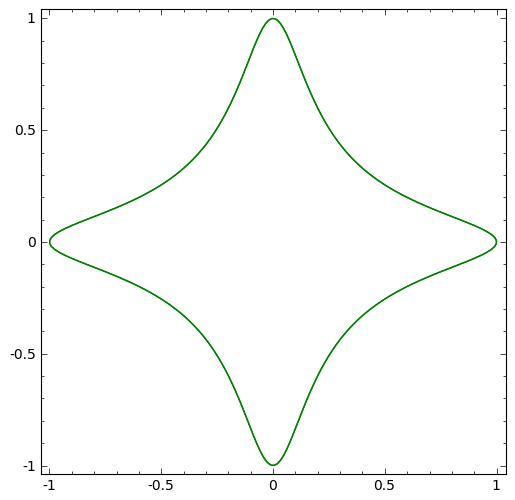
\includegraphics[scale=0.5]{figures/ec1.png}
  \caption{Edwards Curve}
  \label{fig:ec1}
\end{figure}

For the curve in equation \ref{eq:Ed1}, we have the following group law:
\begin{thm}(Edwards Addition Law)
If $a$ is a constant for which $a^5 \ne a$, the formulas
\[
X = \frac{1}{a} \cdot \frac{xy^\prime + yx^\prime}{1 + xyx^\prime y^\prime}
\qquad\qquad
Y = \frac{1}{a} \cdot \frac{yy^\prime - xx^\prime}{1 - xyx^\prime y^\prime}
\]
    describe the addition formula for the elliptic curve 
\[
x^2 + y^2 = a^2 + a^2x^2y^2
\]
\end{thm}
This is theorem (3.1) in \cite{edwards2007normal}; the reader is referred there
    for a proof.
By simple inspection, one can see that the neutral element for this curve is
    $(0, a)$.
Moreover, the inverse $-P$ of the point $P = (x, y)$ is $(-x, y)$:
\begin{align*}
(x, y ) + (-x, y)
    &=  \left( \frac{1}{a} \cdot \frac{xy - yx}{1 - x^2y^2},
               \frac{1}{a} \cdot \frac{y^2 + x^2}{1 + x^2y^2} \right)\\
    &=  \left(0, \frac{1}{a} \cdot \frac{a^2 + a^2x^2y^2}{1 + x^2y^2} \right)\\
    &=  (0, a)
\end{align*}
    using the curve equation in the intermediate step.

As Edwards points out in his proposition (5.1), every curve of the form given
    in equation \ref{eq:Ed1} is \textit{birationally equivalent} to an
    elliptic curve in Weierstrass form.
That is, following Edwards' advice ``to abandon the notion of \textit{points
    of} a curve and to work instead with \textit{rational functions of} a
    curve, one can consider two curves birationally equivalent ``if their
    fields of rational functions are isomorphic.''
We'll discuss this idea in more depth when we go into the details of Bernstein
    and Lange's exploration of Edwards curves.

The addition law given in the above theorem is much simpler than the equivalent
    Weierstrass one given in an earlier section.
There are no special cases, no changing the rules depending on whether $P$ is
    the identity element or $P = -Q$.
We do of course lose the simple geometric description of Weierstrass
    curves\footnote{Though as we'll see in Chapter \ref{chp:pair}, there is
    another geometric interpretation of the group law here.}, but
    that is a small price to pay for so simple, symmetric, and elegant a group
    law.
As we'll see in the next section, the Edwards curve group law's superiority is
    more than just aesthetic: it has desirable consequences for elliptic curve
    cryptographic schemes that use Edwards curves as their group.


\bodysection{Bernstein \& Lange: ECC potential}

In \cite{bernstein2007faster}, Bernstein and Lange generalize Edwards' original
    curve to more cases and turn their attention to cryptographic viability.
First, though, we explain the necessary algebraic geometry.

\bodysubsection{Algebraic Geometry}

Strictly speaking, a curve is ``a projective variety of genus one'' and
    dimension one with a distinguished rational point
    (\cite{silverman2009arithmetic}), so working more in depth with elliptic
    curves requires some understanding of algebraic geometry.
We give a cursory sketch of the necessary pieces based upon
    \cite{silverman2009arithmetic} and \cite{hartshorne1977algebraic}; readers
    who wish for more in-depth coverage of these topics are referred to these
    texts.

First off, in many cases it makes sense to work with projective coordinates (as
    mentioned above) instead of affine ones.
As we saw in the case of Weierstrass curves, sometimes this is not just for
    convenience; we need projective coordinates to be able to discuss the point
    at infinity that arises from adding two points with the same
    $x$-coordinate, for example.
\begin{dfn}
\textit{Projective $n$-space} over a field $K$, denoted by $\mathbb{P}^n(K)$ or
    just $\mathbb{P}^n$, is the set of all $n + 1$ tuples in regular affine
    coordinates
\[
(X_0 , \ldots, X_n) \in \mathbb{A}^{n + 1}
\]
    such that at least one $X_i$ is nonzero, together with the following
    equivalence relation:
\[
(X_0 , \ldots, X_n) \sim (Y_0, \ldots, Y_n)
\]
    if $\exists \lambda \in \overline{K}^\ast$ such that $X_i = \lambda Y_i$
    for each $i$.
We denote an equivalence class by $(X_0 : \ldots: X_n)$, and the individual
    $X_i$ are called \textit{homogeneous} coordinates.
\end{dfn}

Next up is the concept of a \textit{variety}.
Though \cite{silverman2009arithmetic} and \cite{hartshorne1977algebraic}
    subscribe to stricter (or at least more precise) definitions, for our
    purposes the ideas from \cite{adams1994introduction} will suffice.
\begin{dfn}
Given a polynomial $f$ from $\mathbb{P}^n(K)$ to $K$, the \textit{variety}
    $V(f)$ is the set of solutions of the equation $f = 0$.
More formally,
\[
V(f) = \{(X_0 : \ldots: X_n) \in \mathbb{P}^n \mid f(X_0 : \ldots X_n) = 0\}
\]
\end{dfn}

Next we define rational maps between varieties.
\begin{dfn}
Let $V_1, V_2 \subset \mathbb{P}^n$ be projective varieties.
A \textit{rational map} from $V_1$ to $V_2$ is a map of the form
\[
\varphi: V_1 \to V_2, \varphi = (f_0 : \ldots: f_n)
\]
    where the $f_i$ have the property that for every point $P \in V_1$ for
    which all of $f_0,\ldots,f_n$ are defined,
\[
\varphi(P) = (f_0(P): \ldots:f_n(P)) \in V_2
\]
\end{dfn}
Note that a rational map $\varphi: V_1 \to V_2$ need not be a well-defined
    function at every point in $V_1$; however, it may be possible to replace
    each $f_i$ with $gf_i$ for some other rational function $g$ to evaluate
    $\varphi$ at a troublesome point $P \in V_1$.

Finally, we come to birational maps.
\begin{dfn}
A \textit{birational map} is a rational map that admits an inverse; i.e. a
    rational map $\varphi: V_1 \to V_2$ for which there is another rational map
    $\psi: V_2 \to V_1$ such that, when defined, $\varphi \circ \psi$ and $\psi
    \circ \varphi$ are the identity map.
If there is a birational map from a variety $V_1$ to a variety $V_2$, we say
    that these two varieties are \textit{birationally equivalent}.
\end{dfn}
Birational equivalence gives a looser sort of connection between two varieties
    (or curves, since that's what we are focused on) than strict isomorphism.
Basically, two varieties are birationally equivalent if, except for a handful
    of points, they are isomorphic.
In algebraic geometry, singularities of birational maps are typically handled
    by ``blowing up''\footnote{Think ``blowing up a balloon,'' not ``blowing up
    Wile E. Coyote.''} the maps at those points to resolve them.
If a point $(x_0, y_0)$ is a singularity of a map $\varphi$, we can set $y =
    tx$ for some variable $t$ and evaluate what happens as $y \to y_0$.
We'll show an example of this when we discuss binary Edwards curves in Chapter
    \ref{chp:bec}; for more, see a text on algebraic geometry like
    \cite{hartshorne1977algebraic}.


\bodysubsection{Bernstein \& Lange's Edwards Curves}

As the authors mention in the start of \cite{bernstein2007faster}, ``Every
    elliptic curve over a non-binary field is birationally equivalent to a
    curve in Edwards form over an extension of the field, and in many cases
    over the original field.''
Because ``every Edwards curve has a point of order 4,'' to be birationally
    equivalent to a curve without such a point, such as ``the NIST curves over
    prime fields,'' may require working over an extension field.
However, ``to capture a larger class of elliptic curves over the original
    field,'' Bernstein and Lange generalized the definition of Edwards curves
    to the following:
\begin{dfn}
For a fixed field $K$ of characteristic not equal to two, choose $c, d \in K$
    such that $cd(1 - dc^4) \ne 0$ (so $c \ne 0, d \ne 0,$ and $dc^4 \ne 1$).
The \textit{Edwards elliptic curve} or \textit{Edwards curve} defined by $c$
    and $d$ is the (affine) curve of the form
\begin{equation}\label{eq:bled}
x^2 + y^2 = c^2(1 + dx^2y^2)
\end{equation}
\end{dfn}
This definition covers ``more than $\sfrac{1}{4}$ of all isomorphism classes of
    elliptic curves over a finite field,'' so it is a more useful definition
    for our purposes.
Moreover, they show that these are isomorphic to curves where $c = 1$, we will
    stay with the more general form given in \ref{eq:bled}.
From now on we will use this definition when we talk of Edwards curves.
In order to distinguish it from twisted Edwards curves (next section) and
    binary Edwards curves (next chapter), we'll denote the Edwards curve given
    by equation \ref{eq:bled} by $E_{O,c, d}$.

Per theorem (2.1) in \cite{bernstein2007faster}, $E_{O, c, d}$ is birationally
    equivalent to the Weierstrass curve
\[
\left(\frac{1}{1 - dc^4}\right)v^2
    =   u^3 + 2\left(\frac{1 + dc^4}{1 - dc^4}\right)u^2 + u
\]
    via the birational map
\[
(x, y)  \mapsto (u, v)
    =   \left(\frac{1 + y}{1 - y}, \frac{2(1 + y)}{x(1 - y)}\right)
\]
    (since there are only finitely many points with $x(1 - y) = 0$, this is
    indeed a birational map), with inverse
\[
(u, v)  \mapsto (x, y)
    =   \left(\frac{2u}{v}, \frac{u - 1}{u + 1}\right)
\]
    (again, there are only finitely many points such that $(u + 1)v = 0$).

Like Edwards's original formulation, this curve has a simple, symmetric group
    law.
\begin{thm}[Bernstein \& Lange Edwards Addition Law]
For two points $(x_1, y_1)$ and $(x_2, y_2)$ on the Edwards curve $E_{O, c, d}$
    given by equation \ref{eq:bled}, the map
\[
(x_1, y_1), (x_2, y_2) \mapsto
\left(
    \frac{x_1y_2 + y_1x_2}{c(1 + dx_1x_2y_1y_2)}
    ,
    \frac{y_1y_2 - x_1x_2}{c(1 - dx_1x_2y_1y_2)}
\right)
\]
    turns the set of rational points on $E_{O, c, d}(K)$ into an abelian group.
The neutral element for this group law is $\mathcal{O} = (0, c)$, and the
    inverse of the point $(x, y)$ is $(-x, y)$.
\end{thm}
For a proof of this, see theorems (3.1) and (3.2) in
    \cite{bernstein2007faster}.

Critics may wonder why cryptographic researchers are so interested in another
    normal form for elliptic curves.
At first blush, this new normal form may even seem less useful than the
    familiar Weierstrass form since it requires a point of order four.
As we'll see in the last section of this chapter, however, the benefits of
    Edwards curves far outweigh the drawbacks.
For now, though, we'll briefly touch on one other type of Edwards curves.

\bodysubsection{Twisted Edwards Curves}

For the sake of completeness, we now define twisted Edwards
    curves.\footnote{Since they have been the main focus of research for things
    like pairings over Edwards curves; see Chapter \ref{chp:app}.}

In \cite{bernstein2008twisted}, Bernstein et. al. introduced a generalization
    of Edwards curves dubbed ``twisted Edwards Curves.''
These curves ``include more curves over finite fields,'' including ``every
    elliptic curve in Montgomery form'' (another form garnering cryptographic
    interest).
As \cite{arene2011faster} explains, their name ``comes from the fact that the
    set of twisted Edwards curves is invariant under quadratic
    twists\footnote{A \textit{quadratic twist} of a curve is another curve
    isomorphic to it over a field extension of degree two.} while a quadratic
    twist of an Edwards curve is not necessarily an Edwards curve.''

\begin{dfn}
For a field $K$ with $char(K) \ne 2$, and distinct nonzero elements $a, d \in
    K$, the \textit{twisted Edwards curve} $E_{T, a, d}(K)$ is the curve
\[
ax^2 + y^2 = 1 + dx^2y^2
\]
\end{dfn}

As you can see, if $a = 1$, then $E_{T, a, d}$ is an Edwards curve with $c =
    1$.
Furthermore, $E_{T, a, d}$ is a quadratic twist of the Edwards curve $E_{O, 1,
    \sfrac{d}{a}}$
\[
\overline{x}^2 + \overline{y}^2
    =   1 + (\sfrac{d}{a})\overline{x}^2\overline{y}^2
\]
    via the map
\[
(\overline{x}, \overline{y}) \mapsto (x, y)
    =   (\sfrac{\overline{x}}{\sqrt{a}}, \overline{y})
\]
    over the field extension $K(\sqrt{a})$.
Of course, if $a$ is a square in $K$ then these curves are isomorphic over $K$
    itself.

As before, this curve also has a symmetric and elegant group law.
\begin{thm}[Twisted Edwards Addition Law]
Let $(x_1, y_1), (x_2, y_2)$ be two points on the twisted Edwards curve
    $E_{T, a, d}$ given by $ax^2 + y^2 = 1 + dx^2y^2$.
Then the map
\[
(x_1, y_1), (x_2, y_2) \mapsto
\left(
    \frac{x_1y_2 + y_1x_2}{1 + dx_1x_2y_1y_2}
    ,
    \frac{y_1y_2 - ax_1x_2}{1 - dx_1x_2y_1y_2}
\right)
\]
    turns the set of rational points on $E_{T, a, d}(K)$ into an abelian group.
The neutral element for this curve is $(0, 1)$ and the inverse of $(x, y)$ is
    $(-x, y)$.
\end{thm}
For a proof, see \cite{bernstein2008twisted}.

In the next chapter, we'll define binary Edwards curves, a form of elliptic
    curve that is similar in flavor to the above ones except that it is
    defined over fields of characteristic two.
First, though, we'll explain the cryptographic appeal of Edwards curves.

\bodysection{Cryptographic Safety from the Mathematical Foundation}

As one can see from the operation counts given for the explicit formulas for
addition and doubling on Edwards and twisted Edwards curves given in
    \cite{bernstein2007faster} and \cite{bernstein2008twisted}\footnote{Which
    we incorporate into \texttt{e2c2}; see Appendix \ref{chp:src}.}, these new
    curves outperform Weierstrass curves with regards to pure speed.
For abelian groups that form the basis of cryptographic protocols, faster
    computations and more efficiency are certainly very important.
However, binary Edwards curves produce a group law that in pure operation
    counts is a bit slower than its Weierstrass counterpart.\footnote{Slower
    only if we don't take validity checks into account; if we do, per
    \cite{moloneyefficient}, then the binary Edwards group law is still
    competitive.}
As it turns out, the Edwards family of curves is cryptographically interesting
    for a different reason: their groups laws are \textit{unified} and
    \textit{complete}, which leads to implementations that are safer against
    certain types of attacks from the very start; they have greater security
    ``baked into them'' from their mathematical foundation, as it were.

As we mentioned in a previous section, elliptic curve cryptography offers a lot
    of security for relatively low cost because of the lack of subexponential
    algorithms for calculating discrete logarithms.
As such, attackers trying to break ECC implementations tend to focus on the
    technical details of a specific implementation rather than any mathematical
    or algorithmic attacks which may take too long.
Indeed, ``the mathematically proved security of a cryptosystem does not imply
    its implementation [has] security against side-channel attacks,'' as
    \cite{reddy2009elliptic} explains.
A side-channel attack on a cryptosystem implementation is one that attempts to
    gain secret information via measuring some aspect of the implementation's
    performance that, perhaps unknown to its designers or users, leaks such
    information.
Examples for ECC implementations include ``those that monitor the power
    consumption and/or the electromagnetic emanations of a device,''
    \cite{reddy2009elliptic} expands, ``and can infer important information
    about the instructions being executed or the operands being manipulated at
    a specific instant of interest.''
Elliptic curve cryptography with Weierstrass curves is certainly quite
    vulnerable to such attacks;\footnote{At least in the ``textbook'' version
    we've presented, of course.}
The group law as presented in theorem \ref{thm:wgl} has a number of special
    cases one must check for; any implementation needs to check whether either
    of the points it's trying to add is $\infty$, if the two points have the
    same $x$-coordinate but are different points, if they are the same but have
    an $x$-coordinate of zero (so they lie on the same vertical line), or if
    the two points are equal and have a nonzero $x$-coordinate.

There are a multitude of papers detailing such attacks against ECC or trying to
    safeguard systems against them; see \cite{billet2003jacobi,
    brier2002weierstrass, brumley2011timing, chevallier2004low,
    coron1999resistance, goubin2002refined, izu2002exceptional,
    izu2002improved, joye2003elliptic, joye2001hessian, moller2001securing},
    and \cite{okeya2000power} just to name a few.
With all that energy expended on attacking elliptic curve cryptosystems from
    the implementation side, it would certainly be advantageous for a system to
    have a group law that protects against such attacks from the start; this is
    where Edwards curves come in.

As \cite{bernstein2007faster} proves, the group law for an Edwards curve $E_{O,
    c, d}$ is \textit{unified}, since it can also be used to double a point.
That eliminates any need to check whether $P = Q$ when trying to add $P + Q$.
Moreover, this same law works for the neutral element and for inverses; this
    eliminates even more special cases.
Finally, if $d$ isn't a square in $K$ then the addition law is
    \textit{complete}; i.e. it works for all pairs of inputs, and there are no
    special cases to check for at all.
Twisted Edwards curves also share the same cryptographic benefits---the group
    law works for doubling, so it is unified, and is complete if $a$ and $d$
    are both nonsquares in $K$ (i.e. $\sqrt{a}, \sqrt{d} \not\in K$).
To reiterate, this strengthens ECC implementations based on these types of
    curves against side-channel analysis and attacks from the start; the
    elegance of their mathematical theory leads to safer, more easily
    implemented cryptography.
As we'll see in the next chapter, binary Edwards curves also have these
    desirable properties.
